\documentclass[11pt] {article}
\usepackage[margin=1.0in]{geometry}
\usepackage{graphicx}
\usepackage{float}
\usepackage{setspace}
\usepackage{hyperref}
\usepackage [autostyle, english = american]{csquotes}
\MakeOuterQuote{"}

\onehalfspacing
\setlength\parindent{0.5in} % 0.5in indentation

\author{Caleb Jhones}
\date{7 December 2017}
\title{CSCI 250 -- Capstone Project}

\begin{document}
\maketitle

\section*{Abstract}
TODO this needs to be on its own page %TODO

\newpage

\section{Description}
The Raspberry Pi plant watering system is designed to help its user grow healthy plants. Life is very busy and hectic
for everyone these days, and forgetting to water a plant is a death-sentence for anything except the most hardy
vegetation. This system takes that responsibility from the user, and puts it into the hands of a machine which will
never forget to water your plants.

The watering system is very simple to use. Place it near the pot that needs to be watered, and hook up the brass end of
the solenoid to a pressurized water supply. Then plug the 5 volt and 12 volt power supplies into an outlet, and the
Raspberry Pi will boot. As it is set up right now, the Python script needs to be started manually, but for a more permanent
solution it could be started when the Raspberry Pi boots up. In order to start the script manually, use SSH and log into
the Raspberry Pi. Then simply run the script in the background, and then log out.

\begin{figure}[H]
    \begin{centering}
        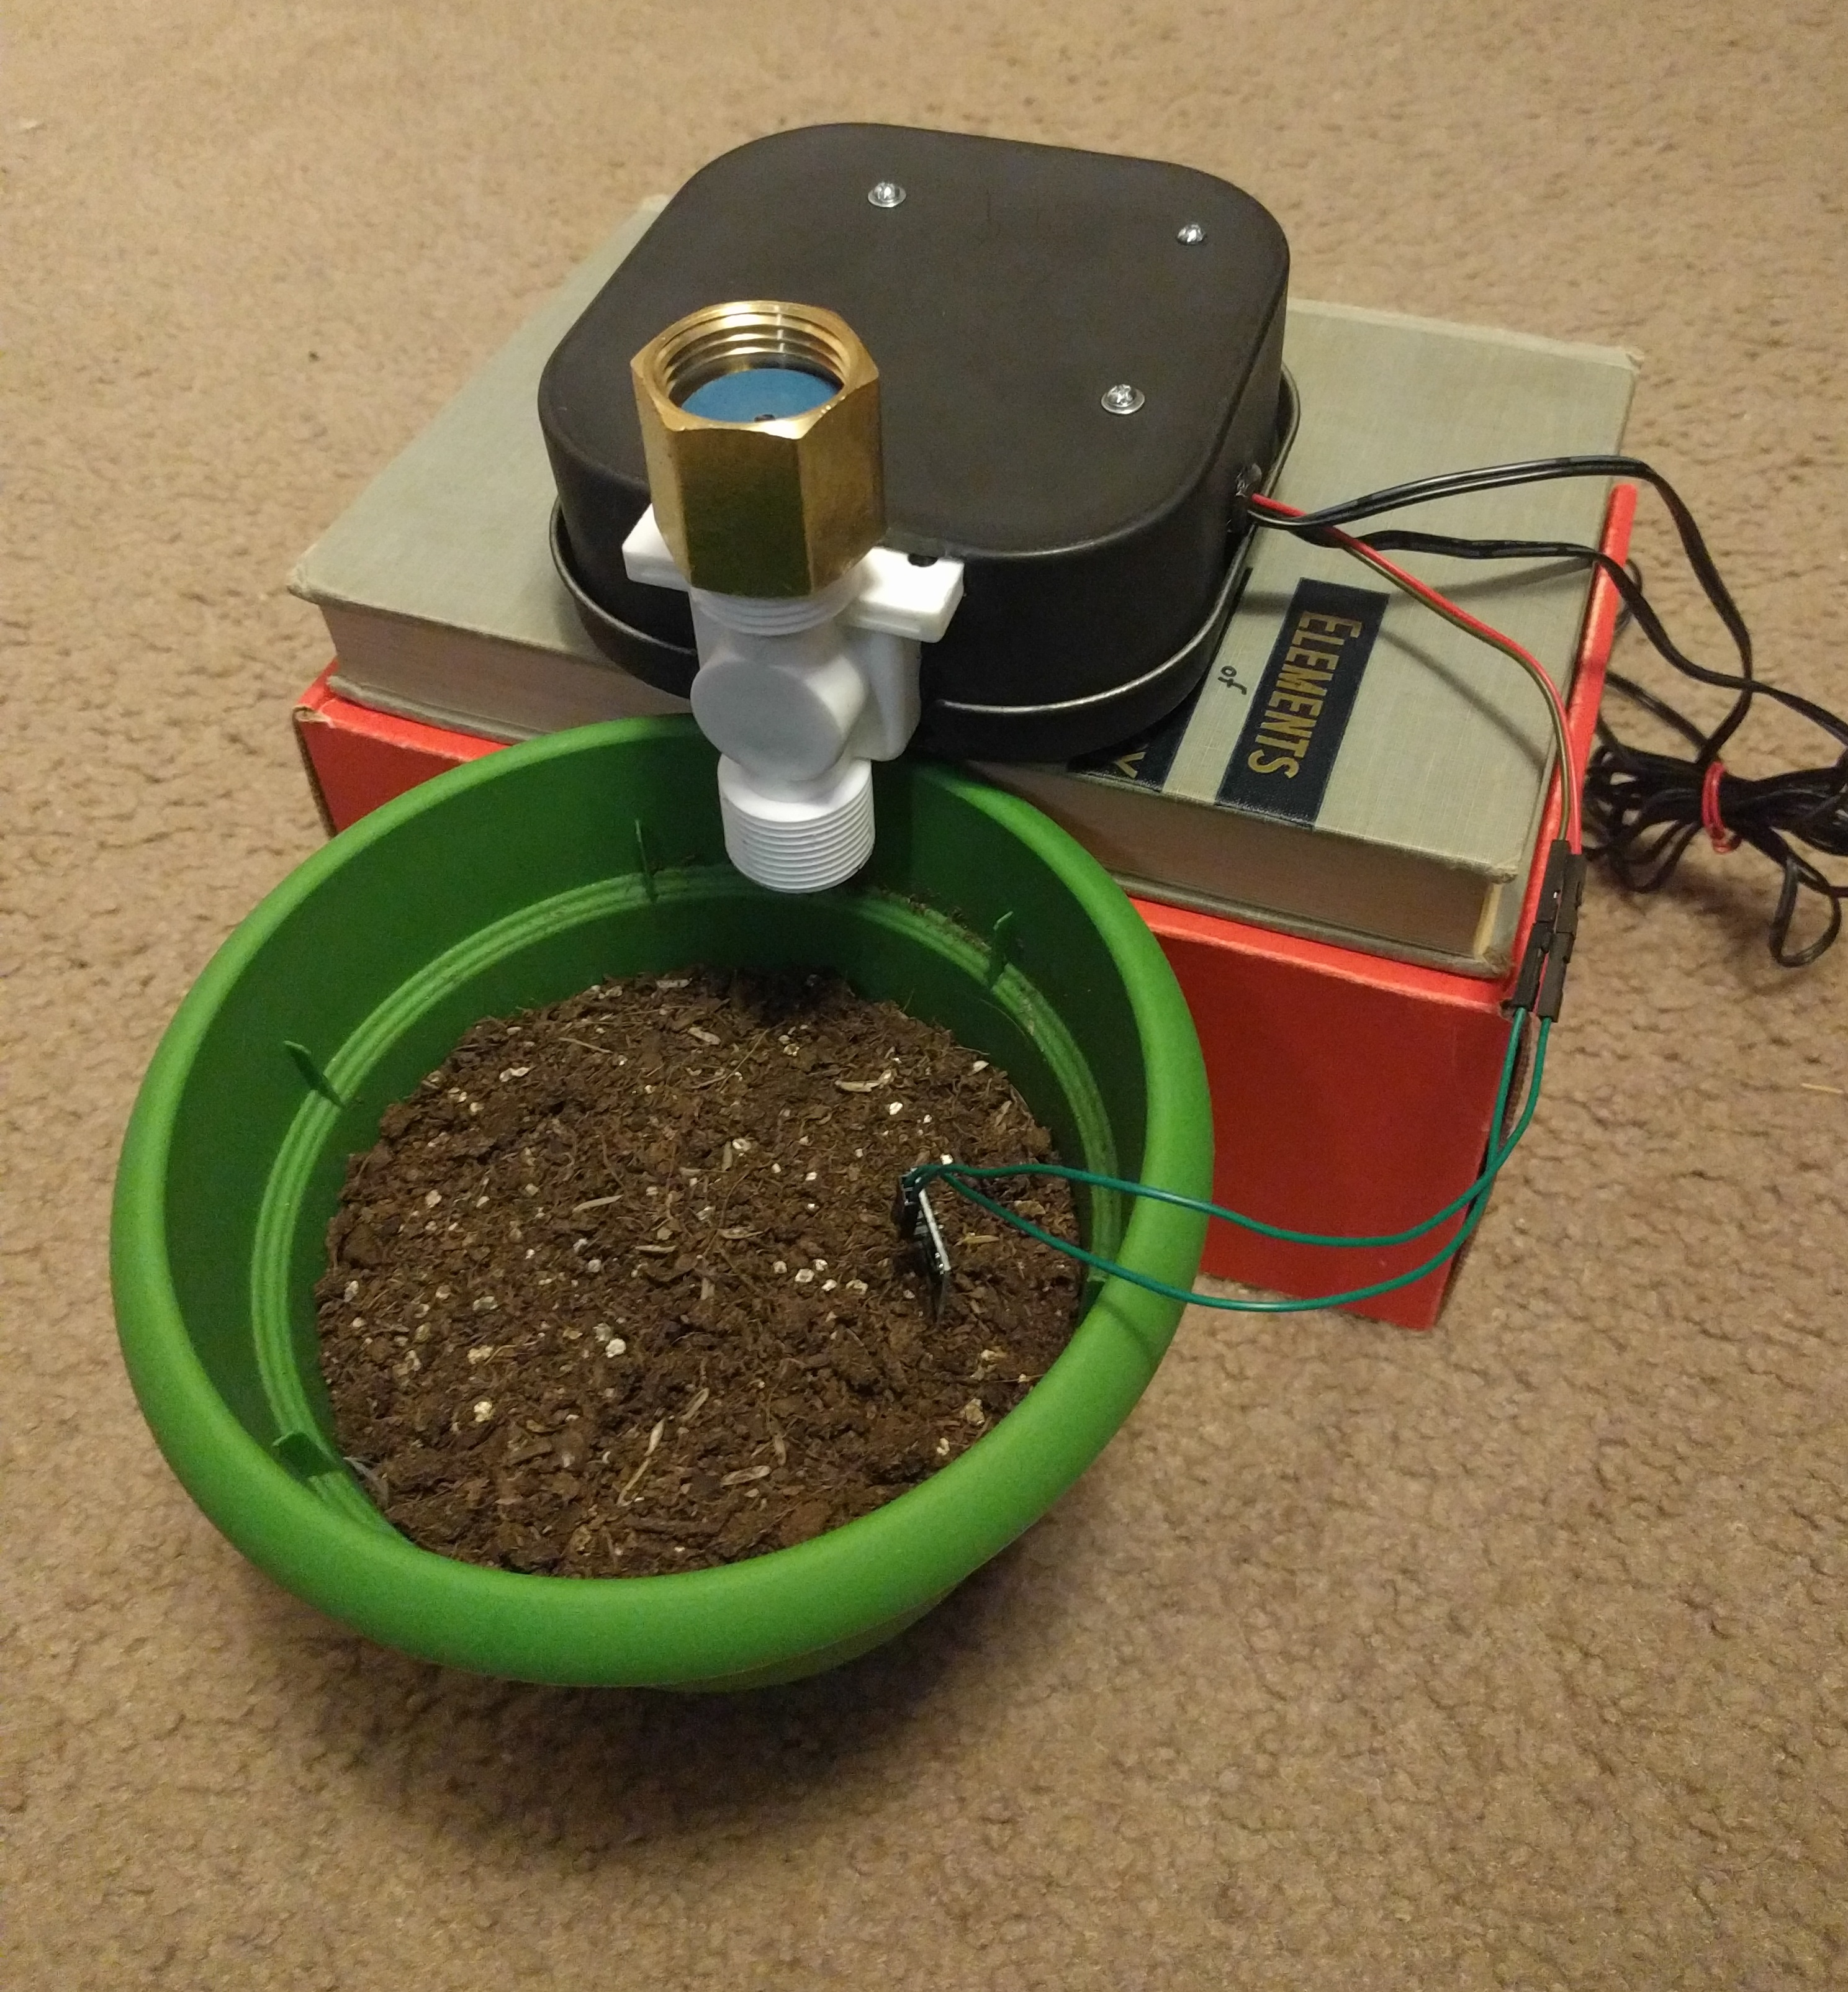
\includegraphics[width=9cm]{../img/in-use}
        \caption{My system in place to water a plant}
    \end{centering}
    \label{in-place}
\end{figure}

The whole system is self-contained in a small box. The box can be opened to easily to service any components that are
inside. All of the wires are easily replaced, as most of them are jumper cables. Those that aren't have connectors that
can be unplugged or plugged in with a screwdriver. See Figure 2 for a look inside the system.

\begin{figure}[H]
    \begin{centering}
        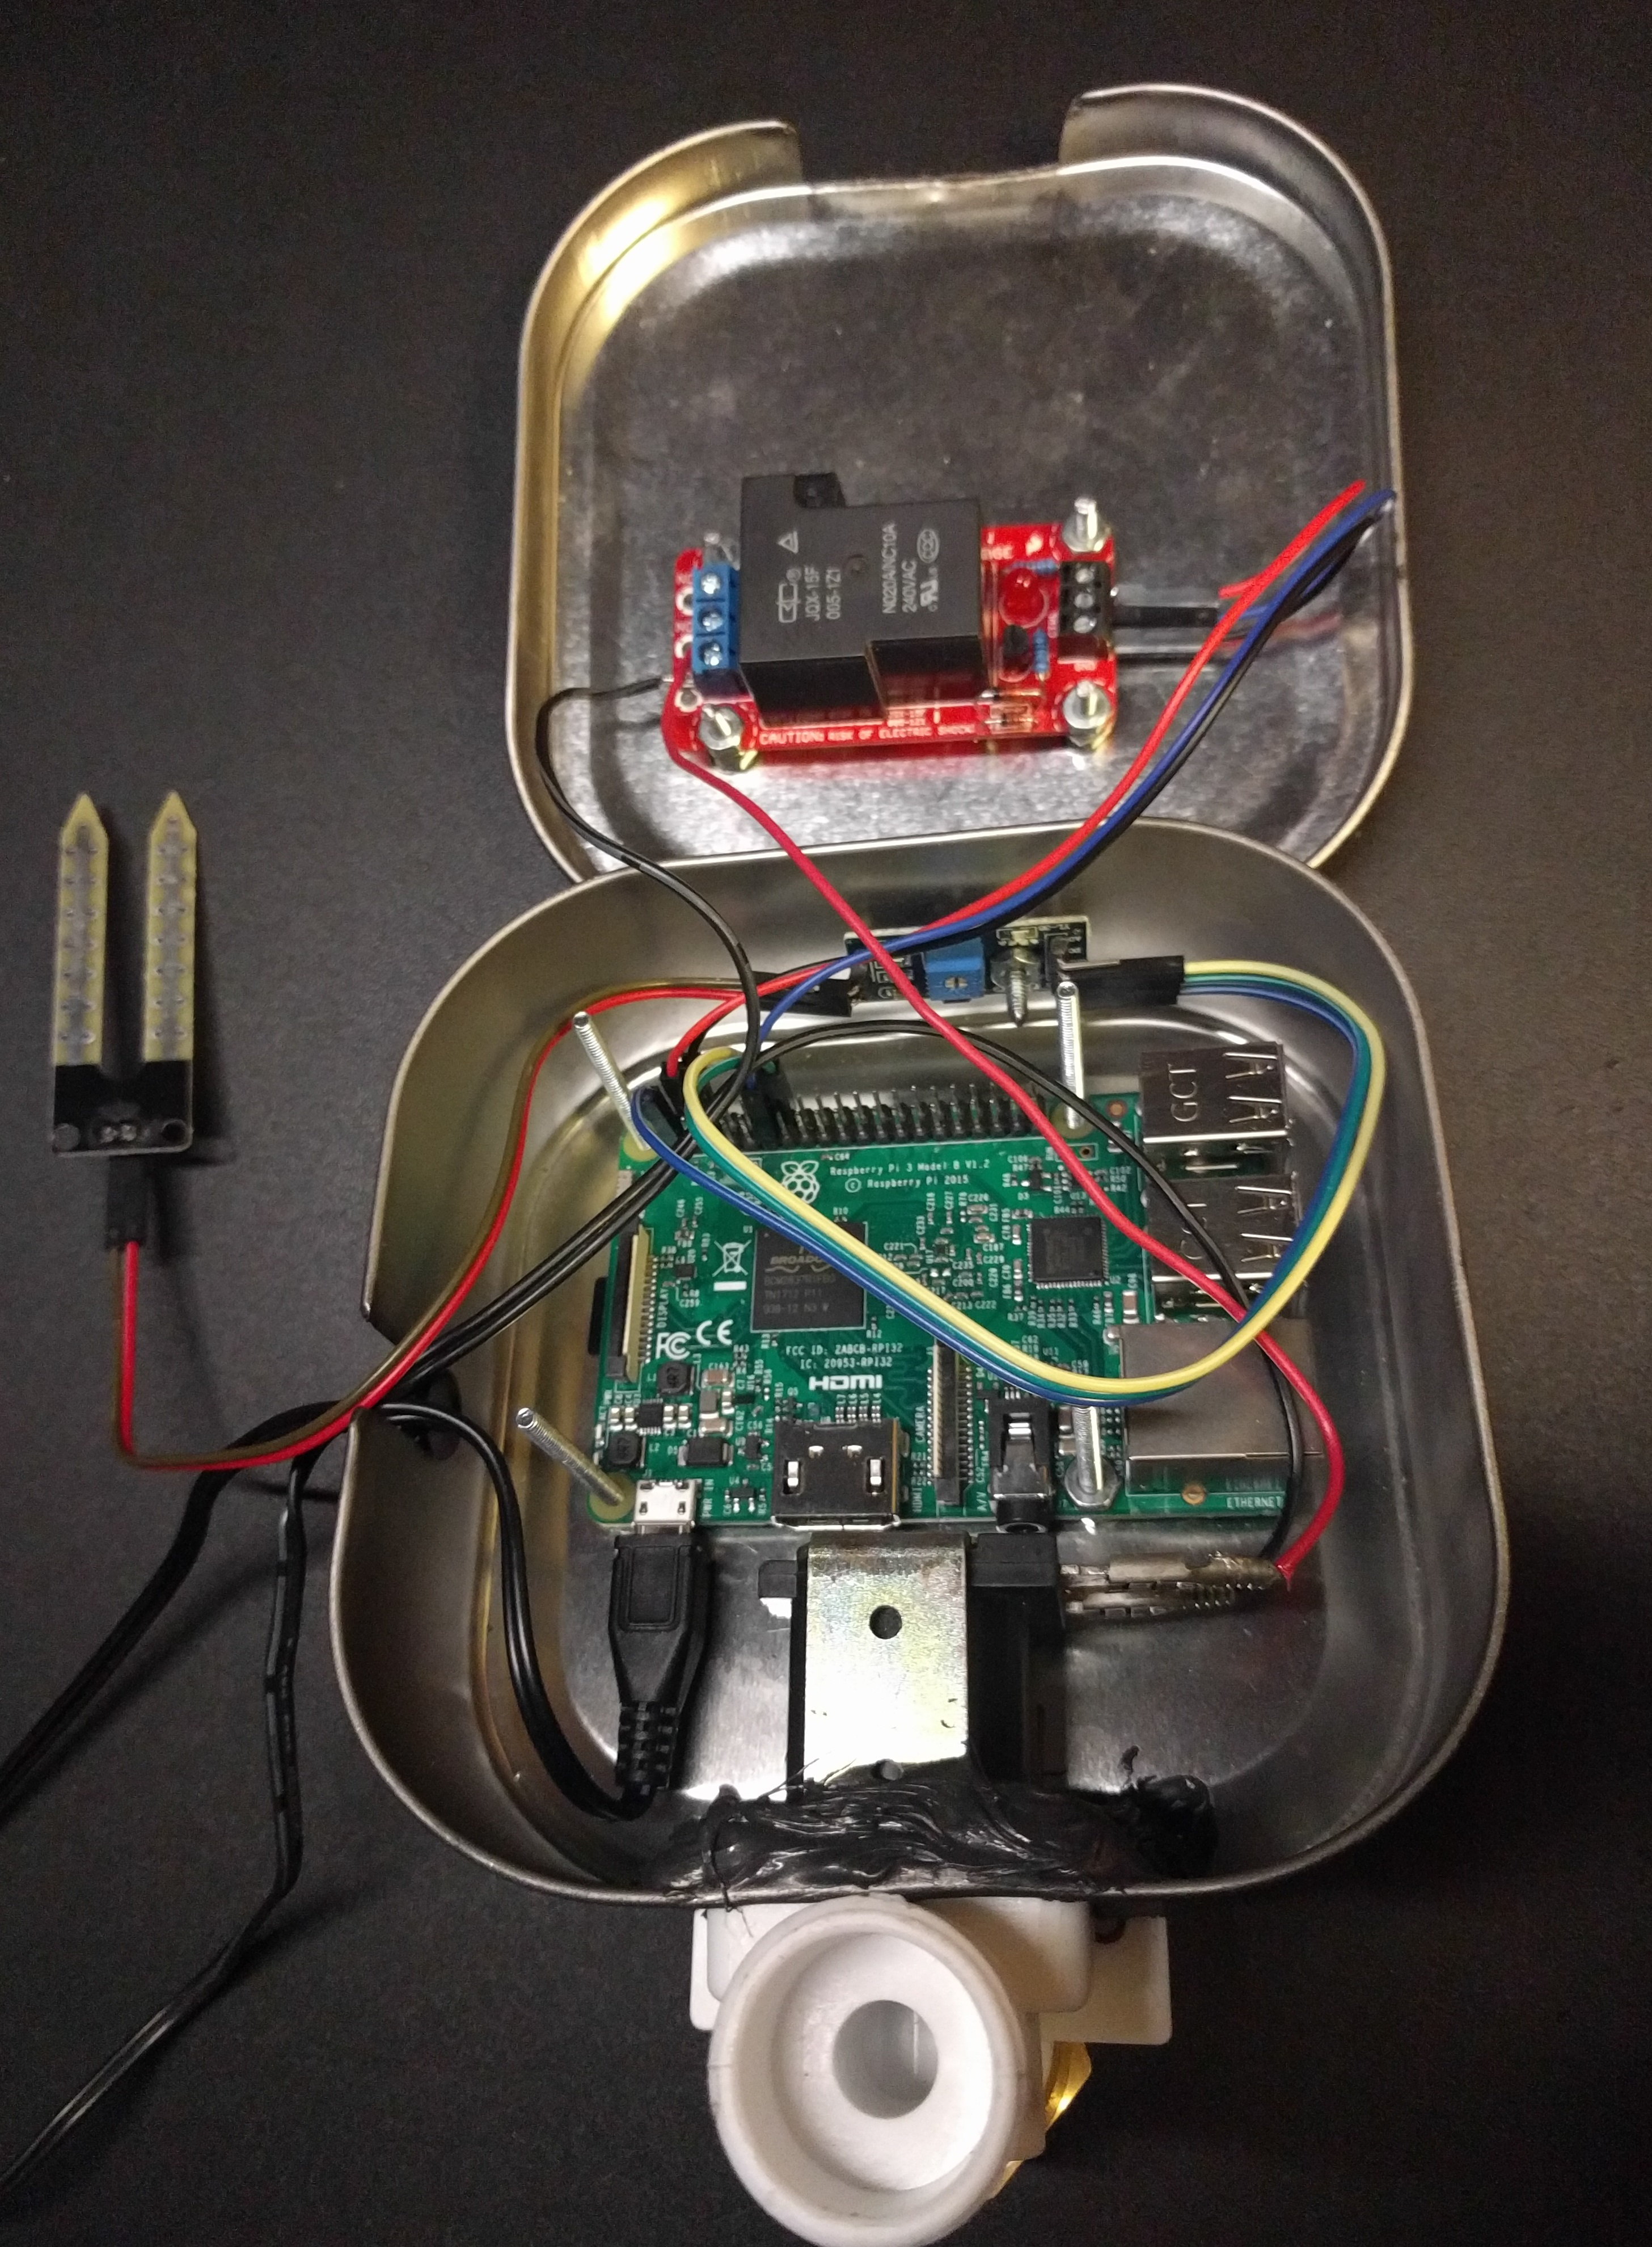
\includegraphics[width=10cm]{../img/the-guts}
        \caption{The inside of the system}
    \end{centering}
    \label{guts}
\end{figure}

\section{Sensors}
The sensor suite is very straight-forward. First, a hygrometer sensor is used to measure the humidity of the soil. This
sensor will read data out in either an analogue or digital format. The digital output is used for this project. This
digital output can be calibrated by a dial on the hygrometer PCB. The hygrometer will read a 1 if the humidity is above
the specified value, and a 0 otherwise. The Raspberry Pi simply reads this 1 or 0 and decides what to do based on it.

I am using a 12 volt solenoid to control water flow. When power is applied to the relay, it pulls a piston back and
lets water flow through the valve. The particular solenoid used in this project needs to be attached to a pressurized
water source. The requirement for pressurized water is because the solenoid piston is spring loaded shut, and requires
high water pressure to push against the spring and open the valve.

The fact that the solenoid is 12 volts means a relay is necessary. The Raspberry Pi operates on 3.3 volts or 5 volts,
but neither of these is sufficient to drive the solenoid. It would also destroy the Raspberry Pi if we tried to push
12 volts through it. The relay is a switch controlled by the 5 volts on the Raspberry Pi, in order to control the 12
volt solenoid. When the Raspberry Pi applies voltage to its side of the relay, it closes the 12 volt side, allowing
current to flow to the solenoid.

See the table for a list of all of the components used, and their approximate prices. The relay and solenoid were
purchased from \href{www.sparkfun.com}{Sparkfun} and the hygrometer was purchased in a pack of 5 from
\href{www.amazon.com}{Amazon}.

\begin{figure}
    \begin{center}
        \begin{tabular}{ | l | c | l | }
            \hline
            Component & Quantity & Price (USD) \\
            \hline \hline
            Raspberry Pi & 1 & 35 \\ \hline
            Hygrometer & 1 & 2 \\ \hline
            Solenoid & 1 & 12 \\ \hline
            Relay & 1 & 15 \\ \hline
        \end{tabular}
        \caption{A list of components and prices}
    \end{center}
\end{figure}

A circuit diagram has been included in Figure 4. It is easy to see the 3.3 volt, 5 volt, and 12 volt pieces of the system.

\begin{figure}[H]
    \begin{centering}
        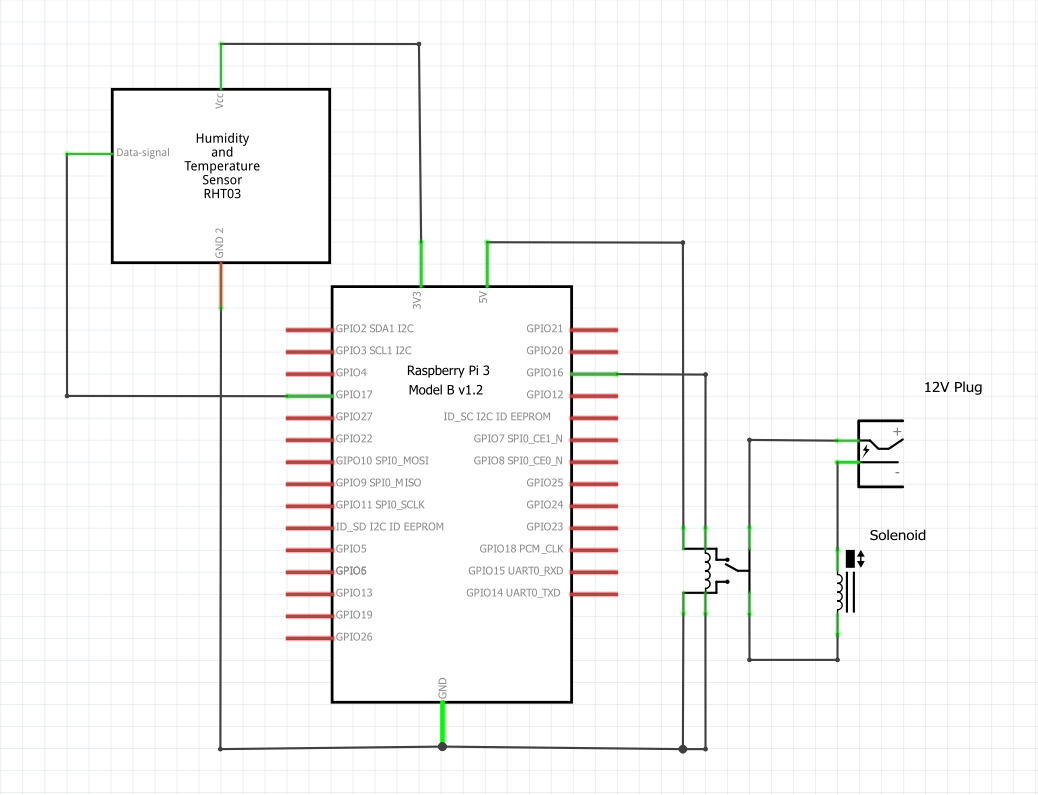
\includegraphics[width=10cm]{../img/circuit}
        \caption{Circuit diagram for the system}
    \end{centering}
\end{figure}

\section{Code}
TODO explain how code works, then have an appendix for the actual code %TODO

\section{Obstacles}
Most of my obstacles revolved around the solenoid. The first issue I ran into was not being able to find a 5 volt unit.
If the solenoid were 5 volts, I could have powered it directly from the Raspberry Pi, removing the need for a relay.
However, as discussed before, the Raspberry Pi cannot run a 12 volt unit, and the relay was added to sit between the
5 volt and 12 volt pieces of the project.

Furthermore, I had initailly wanted to gravity feed the water from a 2 liter bottle on top of the solenoid, but the
need to have pressurized water made this impossible. This fact means the system must have a hose run from a faucet or
water supply of some sort, rather than being self-contained. It also makes it difficult to run the system indoors, as
there are no indoor water sources that can be easily attached to a garden hose. I feel that, for this project to be
used as a permanent solution, finding a better solenoid that can be gravity-fed is a requirement. Connecting the system
to a faucet or similar water supply is impractical.

%TODO more here?

\section{Results}
Overall, the whole build went very smoothly. The electronics hardware was well documented by the individual
manufacturers or retailers, which helped speed the build process along. As far as code is concerned, I wrote small
pieces in test Python files to test coding each sensor individually. For example, I wrote code that would just read
from the hygrometer and print the reading to the screen. This process allowed me to understand each piece in isolation
before moving on to coding the whole system. I feel like this development cycle helped create cleaner and more easily
understandable code.

\section{Future Work}
%find a better solenoid (gravity fed!),
%make there only be 1 power cable (instead of the current 2)
%use an arduino instead,
Going forward, I would like to make the system more usable. This goal would involve a few design changes. The first
change to move toward this goal would be to find a better solenoid. As discussed previously, one which can be gravity
fed is ideal, because it would allow a bottle of water to be used, rather than needing to hook the system into a
faucet.

Having only one power cable, rather than the 2 that the system currently has, would also increase usability. There are
two possible ways to meet this design change. First, if a 5 volt solenoid were used, both it and the Raspberry Pi could
be run off of the same 5 volt power supply. Another option would be to use only the 12 volt supply, and run the
Raspberry Pi's power line from the 12 volt supply through a voltage regulator or a switching mode power supply,
and then to the Raspberry Pi itself. This could cause loading issues, depending on the power draw for the solenoid, so
some caution would need to be taken when setting up this type of system.
% https://niteshbharadwaj.github.io/posts/raspi_from_battery.html

Lastly, I plan to replace the Raspberry Pi entirely. There are small Aduino units based on the Atmel ATtiny85
microcontroller, which draw far less power than the Raspberry Pi. They have 8 pins that can be used for power, digital
inputs and outputs, analogue inputs and outputs, SPI intefacing, and many other applications. These 8 pins are just
enough to drive both the hygrometer and solenoid, which is ideal for this application. Switching the Raspberry Pi out
for a microcontroller also means that the Raspberry Pi would be available for use in other, larger future projects.

%\section{Summary}

\end{document}
